\section{Theory}
\label{sec:theory}

Towards developing a constant space HPYP model and inference procedure we first review dependent PY processes in Section~\ref{sec:dpyp}.  We then develop a dependent hierarchical Pitman Yor process in Section~\ref{sec:dhpyp}.  We show that it is permissible to 


%While the SM model demonstrates promising empirical results \cite{Gasthaus} we are unsatisfied with the linear space requirement for reasons stated earlier.  We propose a framework for limiting the memory required to represent models based on the hierarchical Pitman-Yor process.  Estimation in this framework can be viewed either as a valid inference scheme for a model based on a dependent set of hierarchical Pitman-Yor processes or as an approximate inference technique for a non-varying model.

\subsection{Dependent Pitman-Yor process} 
\label{sec:dpyp}

The $\ES_N(d,c)$ distribution discussed in Section~\ref{basicModel} has a consistency property that is important to us. In the Chinese restaurant metaphor the consistency property corresponds to the fact that if a customer is removed uniformly at random, the remaining customer configuration represents a partition of the integer $N-1$ following the $\ES_{N-1}(d,c)$ distribution.  \cite{???}  This removal of a customer is known as a deletion operation.  Another deletion operation known as size-biased deletion, in which a customer is chosen uniformly at random and all customers seated at the same table are removed from the restaurant, is known to satisfy such a consistency property for the one parameter Ewen's distribution \cite{kingman}.  This is known as the species deletion property \cite{kingman}, but does not hold in the two parameter case \cite{pitman}

The consistency property allows the restaurant representation to be modified to draw samples  $\{ \theta_j^t \}_{i = 1}^{N_t}$ from a sequence of dependent random distributions $\{ \G^t \}_{t=1}^T$ such that 

\begin{eqnarray}
 \label{eqnDependentPY1}  \G^t | d, c, \G_0 &\sim& \PY(d,c,\G_0)\\
 \label{eqnDependentPY2}  \theta_j^t | \G^t &\sim& \G^t \hspace{.5cm} j = 1 \dots N_t.
 \end{eqnarray}
 
We use the index $t$ because of the useful interpretation as time even though it need not be a temporal sequence. The fact that $\G^t_1$ has the same distribution over time is known as stationarity \cite{davis and brockwel}.  
 
The generative procedure, an extension of the analogous procedure for dependent Dirichlet processes \cite{caron}, starts with an empty restaurant and generates $\{ \theta_j^1\}_{i = 1}^{N_1}$ by using the CRP to generate a partition of the integer $N_1$ and then endowing each table with a value drawn independently from $\G_0$.  Between time points customers are deleted uniformly at random from the customer configuration of the restaurant and empty tables are removed from the restaurant.  After the deletion step new customers are seated according to the CRP with the initial customer configuration of the process given by the configuration resulting from the deletion step.  Once new customers have been seated, previously unoccupied tables are endowed with a value drawn independently from $\G_0$.  We set $\theta^t_j = \psi_k$ if  the $j^{th}$ customer seated during the $t^{th}$ time step is seated at table $k$.

If $j$ customers are deleted after time step 1 the partition represented by the starting customer configuration of the restaurant at time step 2 follows a $\ES_{N_1- j}(d,c)$ distribution.  Therefore, after seating new customers in time step 2 the configuration results in partition which follows a $\ES_{N_1 - j + N_2}(d,c)$ distribution.  This is the only result needed to ensure Eqn.~\ref{eqnDependentPY1} and Eqn.~\ref{eqnDependentPY2}.  Note that the number of customers removed from the restaurant between time steps is independent of the consistency result and can thus be either stochastic or deterministic.

Dependence between $\G^t$ is induced by the modified restaurant representation through the undeleted customers.  An exact characterization of the dependence is non-trivial.   \cite{caron} show that in the analogous procedure for dependent Dirichlet distributions, removing fewer customers between time steps induces higher dependence.  In the extreme case of removing all the customers between time steps, the procedure generates samples drawn from independent $\G^t$. Removing no customers implies a $\G$ that is not varying with the index $t$. 

%TODO give graphical model
\subsection{Dependent hierarchical Pitman-Yor Process}
\label{sec:dhpyp}

The mechanism for generating dependent PY processes can be used to generate dependent HPYP as well.  We develop one such strategy for doing so here.  Consider the following model: 

\begin{eqnarray*}
\G_1 | d_1, c_1, \G_0 &\sim& \PY(d_1, c_1, \G_0)\\
\G_2^t | d_2, c_2, \G_1&\sim& \PY(d_2, c_1, \G_1) \hspace{.5cm} t = 1\dots T\\
\theta^t_i | \G_2^t &\sim& \G_2^t \hspace{.5cm} i = 1\dots N_t.
\end{eqnarray*}

A generative procedure giving rise to data from this model is obtained by combining the Chinese restaurant franchise with the modified restaurant process.  The combination executed by removing customers, uniformly at random, from the restaurant corresponding to $\G_2$ between time steps.  The restaurant corresponding the $\G_1$ is unchanged between time steps. At each time, samples are drawn by first producing a partition from the Chinese restaurant franchise using initial restaurant configurations set to the restaurant configurations produced by the deletion step.  After seating the new customers,  previously unoccupied tables are endowed with a parameter $\psi_{2k}$ drawn independently from $\G_1$.  Since we are working in a representation with $\G_1$ analytically marginalized out $\psi_{2k}$ is drawn through the usual method using the CRP and the current customer configuration of the restaurant corresponding the $\G_1$.


\begin{figure}[h!tbp] 
	\begin{center}
		\scalebox{.25}{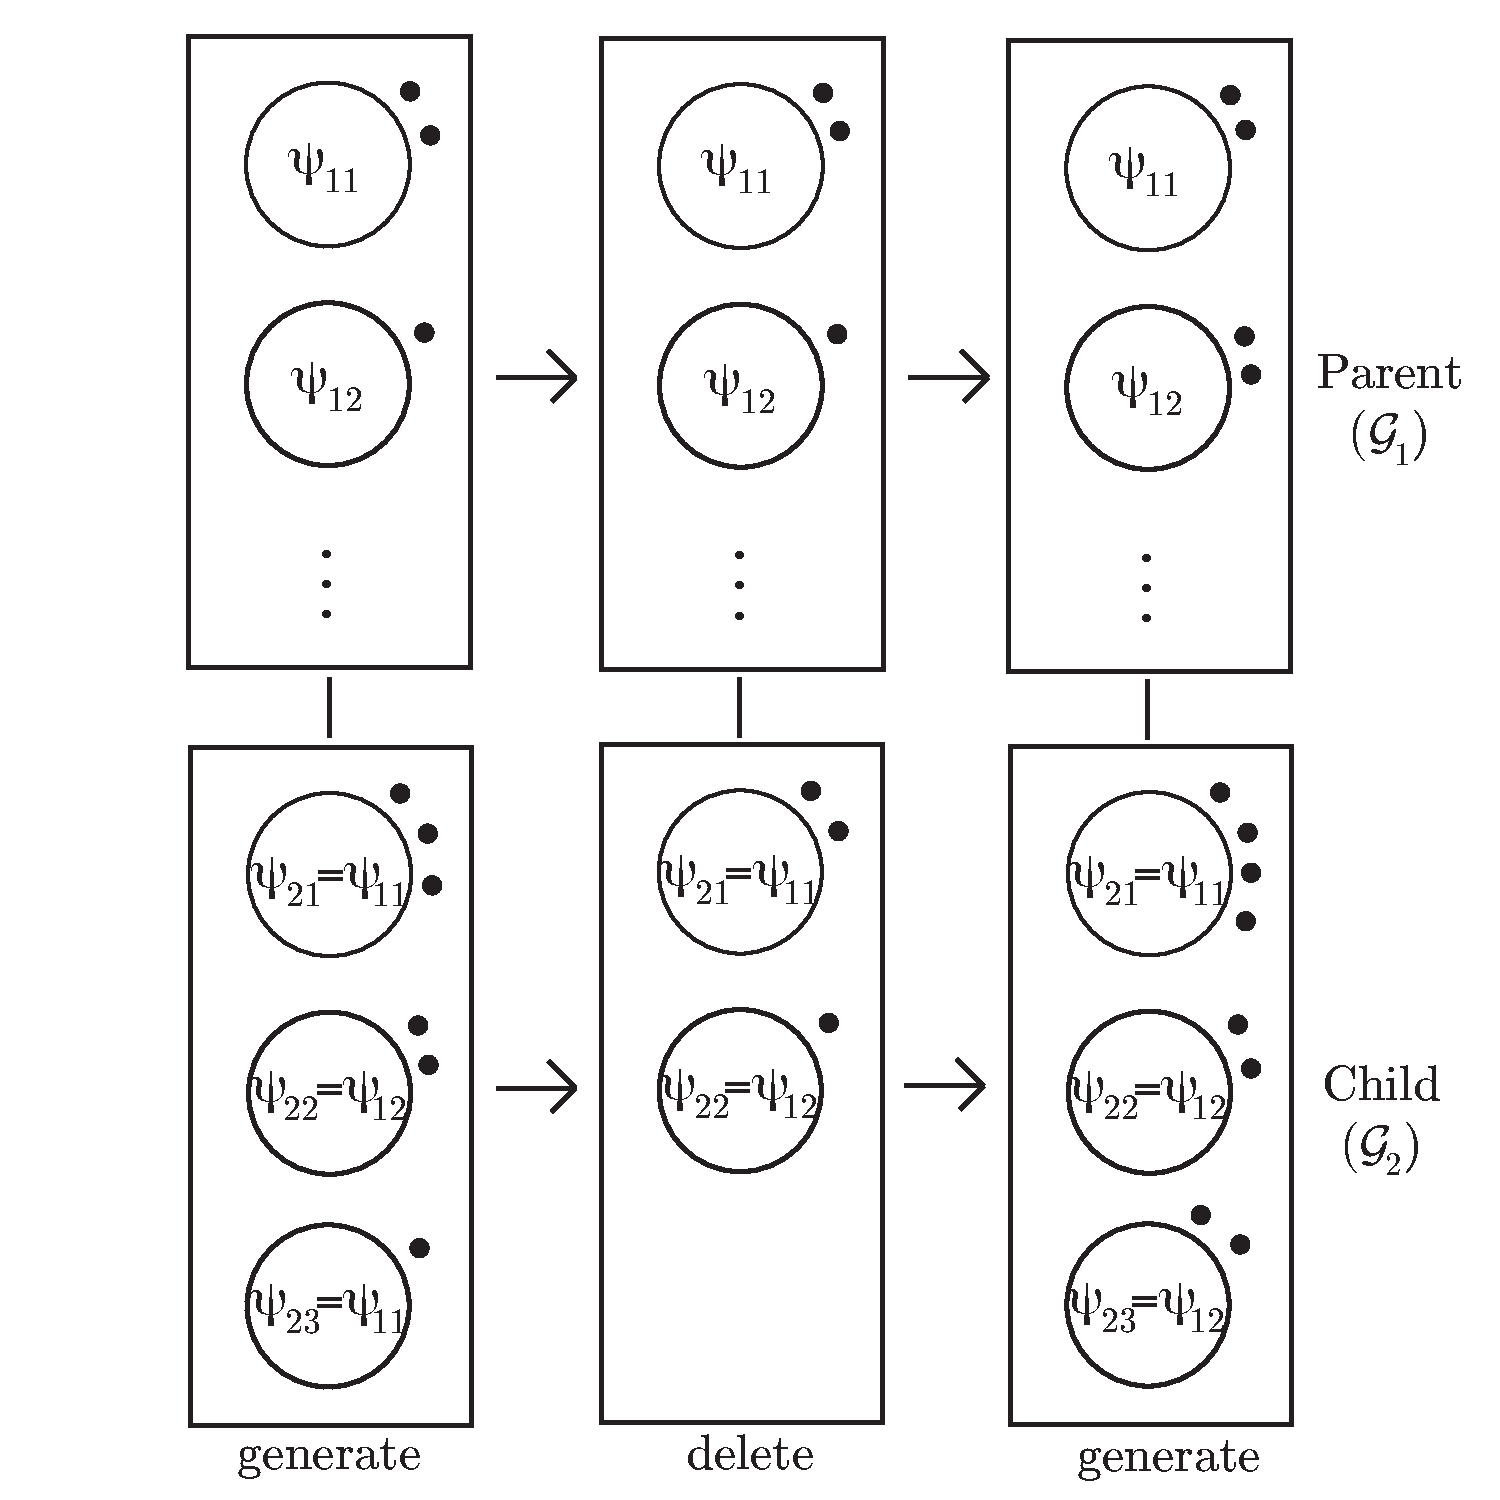
\includegraphics{figure2.pdf}} % [clip=true, viewport= 1in 1in 9in 9in]
		\caption{An example of the possible evolution of the restaurant states in a hierarchical setting}
		\label{figVHPY}
	\end{center} 
\end{figure} 

Figure~\ref{figVHPY} illustrates the potential evolution of the restaurants used during the CRF process modified to draw a sample from dependent distributions following a Pitman-Yor process distribution.  The middle column of restaurants show the restaurant customer configurations after a deletion step.  Note the configuration of the parent restaurant does not change even though one of the tables in the child restaurant has been removed.  The customer configuration in the third column shows a potential seating arrangement which could have generated the observed sample.  Here, a customer was added to the the parent restaurant in order to generate the parameter $\psi_{12}$  given to the third table in the child restaurant.

Simple extensions allowing for dependent distributions higher on the hierarchy are straightforward.  Given the model specification

\begin{eqnarray*}
\G_1^t | d_1, c_1, \G_0  &\sim& \PY(d_1,d_2,\G_0) \hspace{.5cm} t = 1\dots T\\
\G_2^t | d_2, c_2, \G_1^t &\sim& \PY(d_2, c_2, \G_1^t)  \hspace{.5cm} t = 1\dots T\\
\theta^t_i | \G_2^t &\sim& \G_2^t \hspace{.5cm} i = 1\dots N_t, 
\end{eqnarray*}

if we assume independence of the $\{ \G_2^t \}$ we can use the generalized restaurant procedure to generate samples. The assumption of independence indicates that at each time step the restaurant corresponding to $\G_2$ is emptied of all customers. Without the assumption of independence the extension is not straightforward. Creating a modified restaurant procedure to draw a sample from such a model would require a process to update the customer configuration in the restaurant corresponding to $\G_2$ to reflect changes made to the configuration of the restaurant corresponding to $\G_1$, while maintaining a level of dependence.  It is likely that such a process exists, but it is not necessary for this discussion.

\subsection{Bounded memory inference}

The time-varying model will not only allow for a sequence of time-varying distributions, but can also serve to limit the complexity of the model representation. This framework provides a basis for algorithmic control of the complexity of hierarchical Pitman-Yor models like the SM.  As noted earlier, the number of instantiated restaurants in the SM is the fundamental limiting factor regarding memory usage, thus we will consider a single instantiated restaurant as a unit of memory when discussing the model. For the deletion scheme to limit the amount of memory used by the SM model, we must be able to limit the number of instantiated restaurants.

\begin{figure*}[t] 
	\begin{center}
		\scalebox{.4}{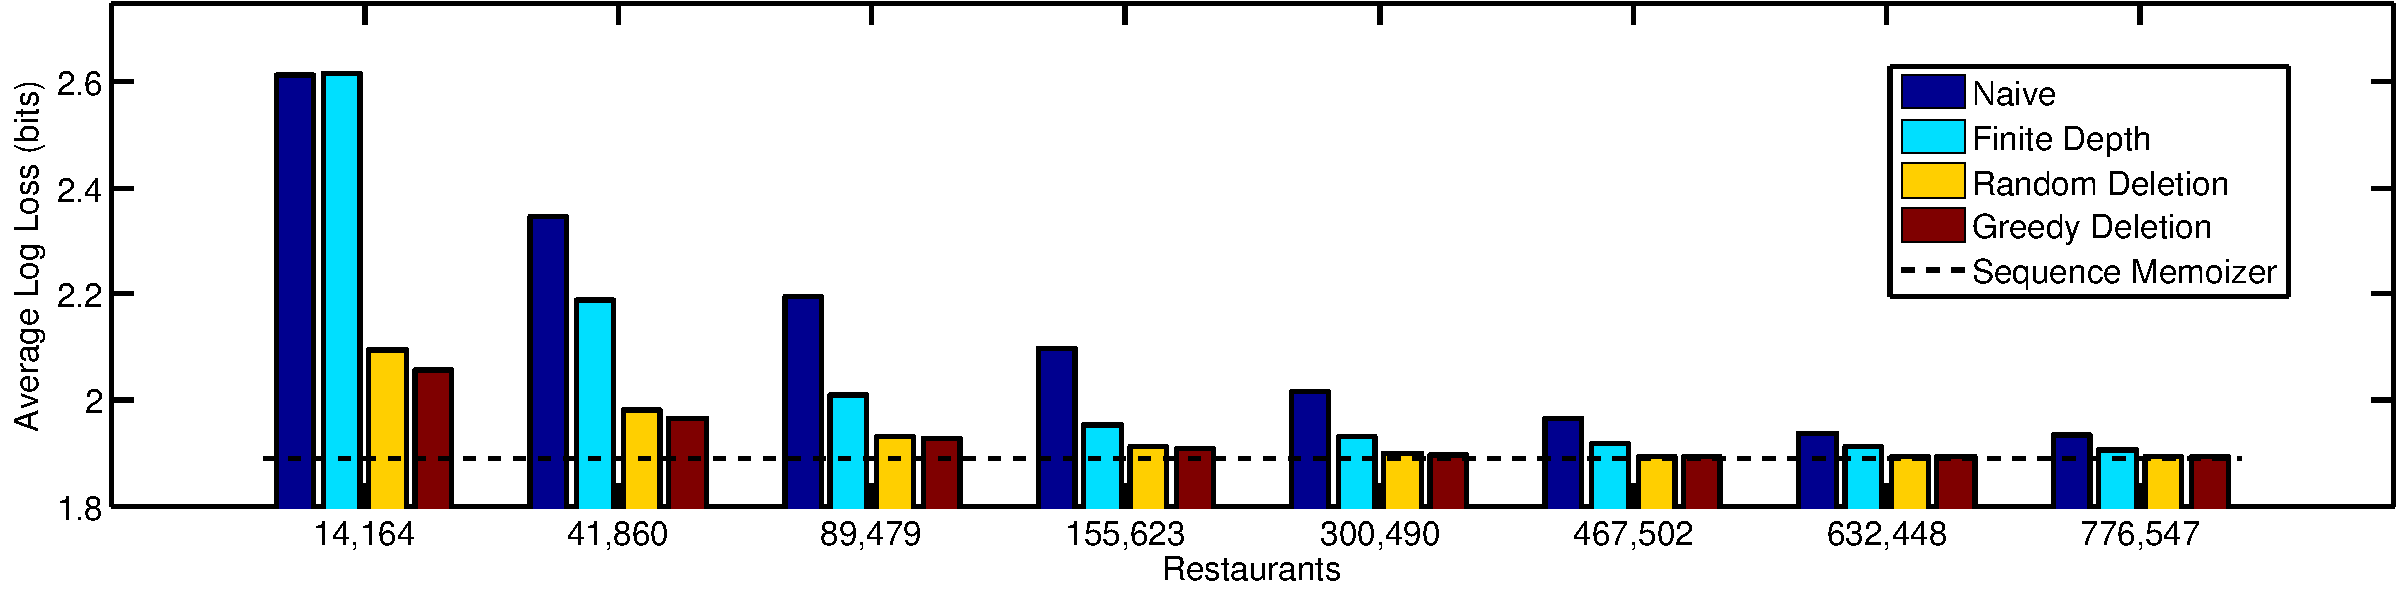
\includegraphics{results_calgary_corpus.pdf}} % [clip=true, viewport= 1in 1in 9in 9in]
		\caption{An example of the possible evolution of the restaurant states in a hierarchical setting}
		\label{figResultsCC}
	\end{center} 
\end{figure*} 

The theory presented above indicates that between time steps we can only delete customers in restaurants at the lowest level.  In the tree which represents the state of the SM, this corresponds to the leaf restaurants.  To achieve memory savings we will need to delete all of the customers at a given restaurant.  Restaurants without people need not be represented in the model state.  This deletion operation gives rise to implicit model assumptions. If, at time step $t$, we delete all the customers in a given leaf restaurant we implicitly assume the distribution over types given the particular context to be independent of the distribution at previous time steps.

\subsection{Bounded memory SM inference}

It is often the case in the SM model that the parent restaurant for a leaf restaurant is not instantiated, thus to actually attain memory savings by deleting a leaf restaurant we must effectively delete all the restaurants in this particular path up until the nearest instantiated restaurant.  The implicit model assumption is that all of the distributions after time $t$ corresponding to those many deleted restaurants are conditionally independent of their previous states.

This is the basic framework for both bounded memory algorithms we present and is the main contribution of this paper.  The assumption that, for many contexts, the distribution changes over time seems appropriate for very long sequences. The assumption of independence required for us to justify our particular deletion process is primarily of practical motivation though we expect information lost to be minimal. 

Finally, we point out that the theory behind these deletion operations holds for general hierarchical Pitman-Yor processes and thus also for finite depth n-gram style models.  In Section~\ref{results} we show some results concerning this type of model as well.
